% TEMPLATE for Usenix papers, specifically to meet requirements of
%  USENIX '05
% originally a template for producing IEEE-format articles using LaTeX.
%   written by Matthew Ward, CS Department, Worcester Polytechnic Institute.
% adapted by David Beazley for his excellent SWIG paper in Proceedings,
%   Tcl 96
% turned into a smartass generic template by De Clarke, with thanks to
%   both the above pioneers
% use at your own risk.  Complaints to /dev/null.
% make it two column with no page numbering, default is 10 point

% Munged by Fred Douglis <douglis@research.att.com> 10/97 to separate
% the .sty file from the LaTeX source template, so that people can
% more easily include the .sty file into an existing document.  Also
% changed to more closely follow the style guidelines as represented
% by the Word sample file. 

% Note that since 2010, USENIX does not require endnotes. If you want
% foot of page notes, don't include the endnotes package in the 
% usepackage command, below.

% This version uses the latex2e styles, not the very ancient 2.09 stuff.
\documentclass[letterpaper,twocolumn,10pt]{article}
\usepackage{usenix,epsfig,endnotes}
\usepackage{listings}
\usepackage{color}
\usepackage{subcaption}

\definecolor{mygray}{rgb}{0.5,0.5,0.5}
\lstset{frame=tb,
  language=Ruby,
  basicstyle={\scriptsize\ttfamily},
  breaklines=true,
  captionpos=b,
  numbers=left,
  numbersep=5pt,
  numberstyle=\tiny\color{mygray},
  xleftmargin=2em,
frame=l,
framexleftmargin=1.5em
}

\usepackage[font=footnotesize,labelfont=bf]{caption}

\begin{document}

%don't want date printed
\date{}

%make title bold and 14 pt font (Latex default is non-bold, 16 pt)
\title{\Large \bf Working Title: Layering is dead, long live layering!}

%for single author (just remove % characters)
\author{
{\rm Your N.\ Here}\\
Your Institution
\and
{\rm Second Name}\\
Second Institution
% copy the following lines to add more authors
% \and
% {\rm Name}\\
%Name Institution
} % end author

\maketitle

% Use the following at camera-ready time to suppress page numbers.
% Comment it out when you first submit the paper for review.
\thispagestyle{empty}


%\subsection*{Abstract}
%Your Abstract Text Goes Here.  Just a few facts.
%Whet our appetites.

\section{Introduction}
\label{sec:intro}

Popular storage systems support diverse storage abstractions by
providing important disaggregation benefits. Instead of maintaining
a separate system for each abstraction, \emph{unified} storage
systems, in particular, support standard file, block, and object abstractions so the same
hardware can be used for a wider range and a more flexible mix of applications. 
As these large-scale unified storage systems evolve to meet the requirements 
of an increasingly diverse set of applications and next-generation hardware, \emph{de jure}
approaches of the past---based on standardized interfaces---are giving way to
domain-specific interfaces and optimizations. While promising, the ad-hoc strategies characteristic of 
current approaches to co-design are untenable.

The standardization of the POSIX I/O interface has been a major success. General adoption
allows application developers to avoid vendor lock-in and encourages storage system
designers to innovate independently. However, large-scale storage systems are generally dominated 
by proprietary offerings, preventing exploration of alternative
interfaces. An increase in the number of special-purpose storage systems characterizes recent history
in the field, including the emergence of high-performance, and highly modifiable, open-source storage systems, 
which enable system changes without of vendor lock-in. Unfortunately, evolving storage system
interfaces is a challenging task requiring domain expertise and predicated on the willingness of
programmers to forfeit the protection from change afforded by narrow
interfaces.

Malacology~\cite{sevilla:eurosys17} is a recently proposed storage system that
advocates for an approach to co-design called \emph{programmable storage}. The
approach is based on exposing low-level functionality as reusable building
blocks, allowing developers to custom-fit their applications to take advantage
of the code-hardened capabilities of the underlying system and avoid
duplication of complex and error-prone services. By recombining existing
services in the Ceph storage system, Malacology demonstrates how two
real-world services, a distributed shared-log and a file system metadata load
balancer, could be constructed using a `dirty-slate` approach. Unfortunately, implementing
applications on top of a system like Malacology can be an ad-hoc process
that is difficult to reason about and manage.

Despite the powerful approach advocated by Malacology, the technique entails navigating 
a complex design space and simultaneously addressing often orthogonal
concerns (e.g. functional correctness, performance, and fault-tolerance).
Worse still, the availability of domain expertise required to build a performant interface is not a fixed or reliable resource. 
As a result, interface composition, as utilized in techniques such as the Malacology Approach, is sensitive to
the change, quickly evolving workloads, and software/hardware upgrades characteristic of unified storage systems.
This necessitates massive maintenance overheads.

To address these challenges, we advocate for the use of high-level declarative
languages (e.g. Datalog) as a means of programming new storage system
interfaces.  By specifying the functional behavior of a storage interface once
in a relational (or algebraic language), optimizers built around cost models
sensitive to storage and access tools and overheads can explore a space of
functionally equivalent physical implementations. Much like query planning and
optimization in database systems, this approach will logically differentiate
correctness and performance and protect higher-level services from lower-level
system changes. However, despite the parallels with database systems, this
paper demonstrates, and begins to address, fundamental differences in the
optimization design space.

In this paper we demonstrate the challenge of programmable storage by showing
the sensitivity of domain-specific interfaces to changes in the underlying
system. We then show that the relational model is able to capture the
functional behavior of a popular shared-log service, and finally we explore
additional optimizations capable of expanding the space of
possible implementations.

\section{Programmable Storage}
\label{sec:progly}

The most common approaches for designing workarounds capable of handling application requirements not met by an underlying storage system roughly fall into among three categories:

{\bf Extra services.} ``Bolt-on'' services are intended to improve performance
or enable a feature, but come at the expense of additional hardware, software
sub-systems, and dependencies that must be managed, as well as trusted.
For instance, such classes of limitations inspired many extensions to Hadoop
~\cite{bu:vldb2010-haloop, ekanayake:hpdc2010-twister,
ekanayake:escience2008-eglmapreduce, mihailescu:hotstorage2012-mixapart}.

{\bf Application changes.} Changing the underlying application with the addition of
 more data management intelligence or via the integration of domain-specific middleware
 represents another popular option for adapting to storage system deficiencies. 
 When application adjustments depend on non-standard semantics exposed by the storage
system (e.g. relaxed POSIX file I/O or MPI-IO hints) the resulting coupling 
can be fragile.
For example, both SchiHadoop~\cite{buck:hpc2011-scihadoop} and Rhea~\cite{gkantsidis:nsdi2013-rhea} do
an excellent jobs of partitioning data in Hadoop applications, but may not
withstand the test of time for future workloads, since the partitioning is
specific to scientific data.

{\bf Storage modifications.} When these two approaches fail to meet an
application's needs, developers may turn their attention to any number of
heavyweight solutions ranging from changing the storage system itself, up to
and including designing entirely new systems. This approach can require
significant cost, domain knowledge, and extreme care when building or
modifying critical software that can take years of code-hardening to trust.
For example, HDFS fails to meet many needs 
of metadata-intensive workloads~\cite{shvachko:login2012-hdfs-scalability}.
Systems builder achieve performance improvement by modifying the underlying
architecture or API~\cite{balmin:sigmod2012-clydesdale}.

Rather than relying on storage systems to evolve or applications to
change, the ``Malacology Approach''
manifests a hybrid technique which embraces interface instability without placing
an unmanageable burden on developers.

\subsection{The Malacology Approach}

%\textcolor{red}{HELP! We can't decide if this section should be called ``The
%Programmable Storage Approach" or ``The Malacology Approach" -- I argue that
%Malacology is the prototype but Noah thinks Malacology Approach makes more
%sense.}

Programmable storage systems improve the development experience over the lifecycles of long-lived and co-designed applications
and storage systems by exposing a number of existing internal services capable of principled composition. Importantly, the compositionality of the internal functionality aids in the development of higher-level application specific services~\cite{sevilla:eurosys17}.
Figure~\ref{fig:malacology} shows the architecture of Malacology, a prototype programmable storage system
implemented in Ceph, which exposes a variety of low-level internal services
such as custom object interfaces, cluster metadata management, and
load-balancing. While Ceph natively exposes file, block, and object
abstractions, Malacology demonstrates the construction of two real-world
services (ZLog~\cite{watkins:ucsc-soe-16-12} and Mantle~\cite{sevilla:sc15-mantle}) using only the composition of existing interfaces present in Ceph.

\begin{figure}[t]
\centering
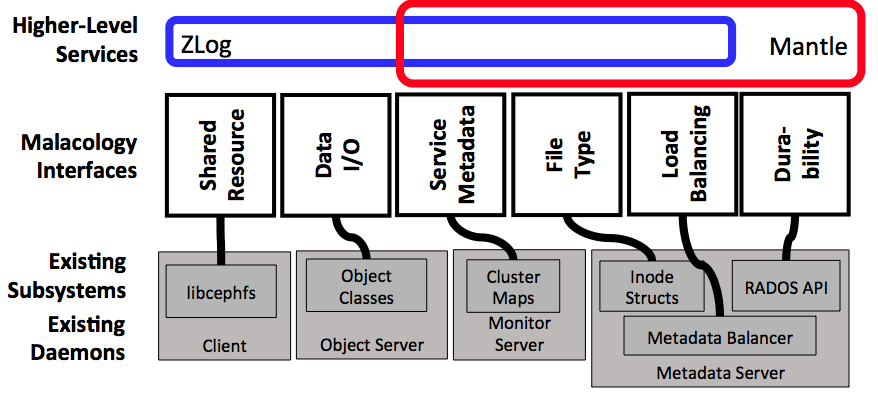
\includegraphics[width=1.0\linewidth]{implementation-overview.png}
\caption{Malacology implementation in Ceph. Existing sub-systems are composed
    to form new services and application-specific optimizations.}
\label{fig:malacology}
\end{figure}

ZLog is a high-performance distributed shared
log that implements the CORFU protocol~\cite{balakrishnan:nsdi12}.
This protocol achieves high-throughput by using a soft-state network-attached
counter and stripes log content over a cluster of flash devices exposing
protocol-specific storage interfaces. While CORFU is a stand-alone system,
Malacology is able to instantiate the same abstraction and approximate 
the same unique optimizations.

Malacology reproduces the CORFU network-attached counter service using a
capability-based mechanism found in the Ceph distributed file system for
managing cached metadata. ZLog implements the counter using the metadata server's ability to provide temporary
exclusive access to a shared resource (in this case, file metadata).  In ZLog, CORFU's storage device interface is
constructed using application-specific object interfaces in Ceph. These
software-based interfaces are constructed as a composition of low-level I/O
interfaces (e.g. an LSM-tree and a bytestream) operating in an atomic
context. The technique allows the interface to maintain consistency across native
interfaces.

The demonstration of interface synthesis in Malacology suggests a new form of
application development capable of significantly reducing the number of lines of code associated with a higher-level application.
While such an ability to construct software-defined interfaces is powerful,
subsequent analyses demonstrate how access to low-level interfaces can be a double-edged
sword providing extended application development powers at the cost of increased maintenance complexity.

\section{Design Space}
\label{sec:dspace}

The narrow interface exposed by storage systems has been a boon in allowing
systems and applications to evolve independently, in affect limiting the size
of the design space where applications couple with storage. Programmable
storage lifts the veil on the system, and with it, forces applications developers
to confront a large set of possible designs.

\subsection{Software Parameters}

To illustrate the design space challenge we implemented as an object interface
the CORFU storage device specification, that is a write-once interface over a
64-bit address space. The interface is used as a building block of the CORFU
protocol to read and write log entries that are striped over an entire
cluster.  The implementations differ in their optimization strategy of
utilizing internal system interfaces. For instance one implementation uses a
key-value interface to manage the address space index and entry data, while
another implementation stores the entry data using a byte-addressable
interface.

\begin{figure}[t]
\centering
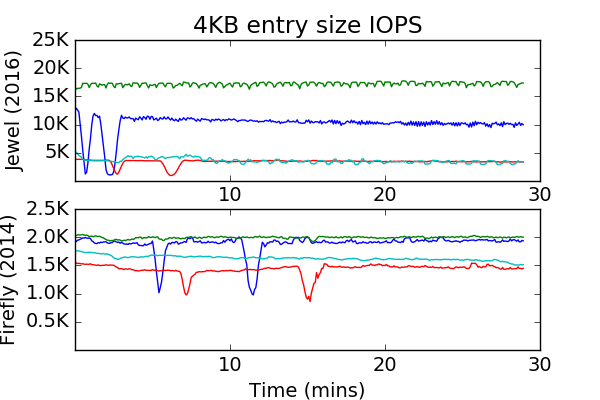
\includegraphics[width=1.0\linewidth]{jewel_v_firefly_pd.png}
\caption{asdf}
\label{fig:phy-design}
\end{figure}

Figure~\ref{fig:phy-design} shows the append throughput of four such
implementations run on two versions of Ceph from 2014 and 2016. The first
observation to be made is that performance in general is significantly better
in the newer version of Ceph. However, what is interesting is the relationship
between the implementations. Run on a version of Ceph from 2014, the top two
implementations perform with nearly identical throughput, but have strikingly
different implementation complexities. The performance of the same
implementations on a newer version of Ceph illustrate a challenge: given a
reasonable choice of a simpler implementation in 2014, a storage interface
will perform worse in 2016, requiring significant rework of low-level
interface implementations.

\textbf{Takeaway}: Choosing the best implementations is dependent on both the
timing of the development (Ceph Version) and the expertise of the
administrator (Ceph Features). Ceph development is a moving target with
multiple stable releases each year, 400+ contributors, and 70--260 commits per
week.  Disruptive and innovative change in Ceph is also common place, with
features such as BlueStore~\cite{weil:vault2016-bluestore} replacing
traditional file systems like XFS that have limitations on the workloads
generated by Ceph such as double writes and metadata scalability. 

\subsubsection{System Tunables}

The most recent version of Ceph (v10.2.0-1281-g1f03205) has 994 tunable
parameters\footnote{This number comes from \texttt{src/common/config\_opts.h}
with debug options filtered out.}, where 195 of them pertain to the OSD itself
and 95 of them focus on the OSD back end file system (i.e. its
\texttt{filestore}). Ceph also has tunables for the subsystems it uses, like
LevelDB (10 tunables), RocksDB (5 tunables), its own key-value stores (5
tunables), its object cache (6 tunables), its journals (24 tunables), and its
other optional object stores like BlueStore (49 tunables).

This many domain-specific tunables makes it almost impossible to come up with
the best set of tunables, although auto-tuning like the work done
in~\cite{behzad:sc2013-autotuning} could go a long way. Regardless of the
technique that we use, it is clear the number of tunables increases the
physical design parameters to an unwieldy state space size.

\textbf{Takeaway}: the number and complexity of Ceph's tunables makes
brute-force parameter selection hard.

\subsubsection{Hardware Parameters}

Ceph is designed to run on a wide variety of commodity hardware as well as new
NVMe devices. All these devices have their own set of characteristics and
tunables (e.g., the IO operation scheduler type). In our experiments, we tested
SSD, HDDs, NVMe devices and discovered a wide range of behaviors and
performance profiles. As an example, Figure~\ref{fig:jewel-hdd-128b} shows the
write performance of 128 byte log entries using Jewel and a single HDD.
Performance is 10\(\times\) slower than its SSD counterpart in
Figure~\ref{fig:jewel_v_firefly_v_es} (top row, third column) but the behavior
and relative performance make this hardware configuration especially tricky.

The behavior of the 1:1 implementations shows throughput drops lasting for
minutes at a time -- this limits our focus to the N:1 implementations. The
performance of \texttt{(N:1, BS)} implementation is almost identical to
\texttt{(N:1, KV)} (within 1\% mean throughput). Regardless of the true
bottleneck, it is clear that choosing \texttt{(N:1, KV)} is the better choice
because of the resulting implementation should be less complex and there is
minimal performance degradation.

\textbf{Takeaway}: choosing the best implementations is dependent on hardware.
Something as common as an upgrade from HDD to SSD may nullify the benefits of a
certain implementation. 

\section{Declarative Programmable Storage}
\label{sec:prog-model}

Current ad-hoc approaches to programmable storage restrict use to developers
with distributed programming expertise, knowledge of the intricacies of the
underlying storage system and its performance model, and primarily use
hard-coded imperative methods. This restricts the use of optimizations that
can be performed automatically or derived from static analysis.  Based on the
challenges we have demonstrated stemming from the dynamic nature and large
design space of programmable storage, we present an alternative, declarative
programming model that can reduce the learning curve for new users, and allow
existing developers to increase productivity by writing less code that is more
portable.

The model we propose corresponds to a subset of the Bloom language which is a
declarative language for expressing distributed programs as an unordered set
of rules~\cite{alvaro:cidr11}. These rules fully specify program semantics and
allow a programmer to ignore the details associated with how a program is
evaluated. This level of abstraction is attractive for building storage
interfaces whose portability and correctness is critical. We model the
storage system state uniformly as a collection of relations, with interfaces
being expressed as a collection of \emph{queries} over a request stream that
are filtered, transformed, and combined with system state. Next we present a
brief example of the CORFU shared-log interface expressed using this model.

\subsection{Example: The CORFU Log Interface}

The CORFU log protocol achieves high-performance in part by striping the log
across a large number of fast storage devices. Using our declarative language
we model the log as a single relation, hiding the implementation detail of log
partitioning. Lines 2-3 in Listing~\ref{lst:corfublm} show the declaration of
state for the CORFU interface consisting of two persistent collections: one for
the log data, and one for interface metadata. The mapping of collections onto
physical storage is abstracted at this level, permitting optimizations
discussed earlier to be discovered and applied transparently by an optimizer.
Line 5 defines the write operation as a scratch collection with models
non-persistent state only valid for the duration of a single time stemp
allowing an optimizer to treat this state as volatile.

\begin{lstlisting}[caption={Sample \emph{corfu.bloom} program listing}, label=lst:corfublm]
bloom :corfu do
  table :epoch, [:epoch]
  table :log, [:pos] => [:state, :data]
  scratch :write_op, op.schema
end
bloom :write do
  temp :valid_write <= write_op.notin(found_op)
  log <+ valid_write{|o| [o.pos, 'ok', o.data]}
  ret <= valid_write{|o| [o.type, o.pos, o.epoch, 'ok'] }
  ret <= write_op.notin(valid_write) {|o| ['read-only'] }
end
bloom :trim do
  log <+- trim_op{|o| [o.pos, 'trimmed']}
  ret <=  trim_op{|o|
    [o.type, o.pos, o.epoch, 'ok']}
end
\end{lstlisting}

The write-once 64-bit address space exposed by CORFU storage devices depends on
a method for quickly resolving the log position to metadata and physical
storage addresses. The declarative specification of the write interface shown
on lines 8-13 is expressed independently of the implementation and any
optimization strategies.  In addition, the CORFU interface depends on a trim
interface to mark unused poritions of the log (shown on lines 10-15) Trimmed
entries are tracked as unused for reclamation, and implementations may take
advantage of specific optimizations provided by an index implementation or
hardware support found in modern non-volatile memories.

\begin{figure}
\centering
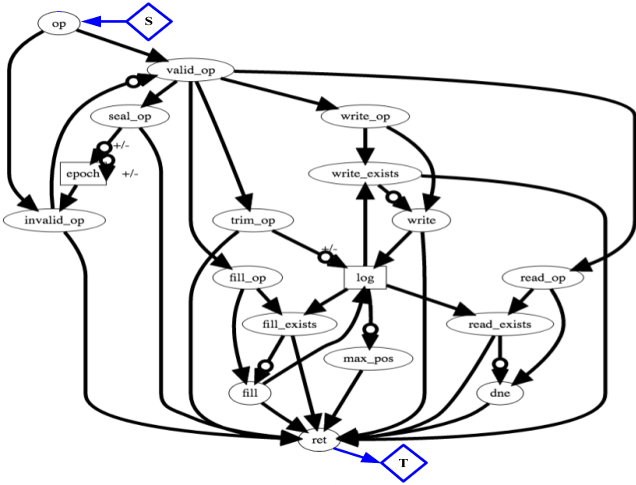
\includegraphics[width=0.7\columnwidth]{Corfu_viz_expanded2.png}
\caption{Dataflow graph for the CORFU interface written in Bloom}
\label{fig:flow}
\end{figure}

Amazingly, only a few code snippets can express the semantics of the entire
storage device interface requirements in CORFU\footnote{Due to space
limitations refer to \cite{watkins:ucsc-soe-16-12} for a full program
listing.}.  Figure~\ref{fig:flow} shows the dataflow diagram for the entire
CORFU program expressed in Bloom that can serve as input to an optimizer.
Beyond the convenience of writing less code, it is far easier for the
programmer writing an interface such as CORFU to convenience herself of the
correctness of the high-level details of the implementation without being
distracted by issues related to physical design or the many other gotchas that
one must deal with when writing low-level systems software.

%For reference our prototype implementation of CORFU in Ceph (called
%ZLog\footnote{https://github.com/noahdesu/zlog}) is written in C++ and the
%storage interface component comprises nearly 700 lines of code, and uses a
%hard-coded indexing strategy that has been rewritten multiple times to explore
%alternative optimization techniques.

%\begin{figure}[t]
%\begin{subfigure}{.2\columnwidth}
%\centering
%\scalebox{0.4}{
%\begin{tikzpicture}[->,>=stealth',shorten >=1pt,auto,node distance=2.2cm,semithick]
%%\tikzstyle{every state}=[fill=red,draw=none,text=white]
%
%  \node[initial left,state] (A)              {$EG$};
%  \node[state]         (B) [below right of=A] {$CP$};
%  \node[state]         (D) [right of=B]       {$IO$};
%  \node[state]         (C) [above right of=A] {$GC$};
%  \node[state]         (E) [right of=C]       {$US$};
%  \node[state]         (F) [below right of=E] {$Out$};
%
%  \path (A) edge        node [left] {R,W,F} (B)
%            edge        node {T}     (C)
%        (B) edge        node {F}     (C)
%            edge        node {R,W}   (D)
%        (C) edge        node {F,T}   (E)
%        (D) edge        node {W}     (E)
%            edge        node {R}     (F)
%        (E) edge        node {F,T,W} (F);
%\end{tikzpicture}
%}
%\caption{}
%\label{fig:corfu-sm}
%\end{subfigure}\hfill
%\begin{subfigure}{.6\columnwidth}
%\centering
%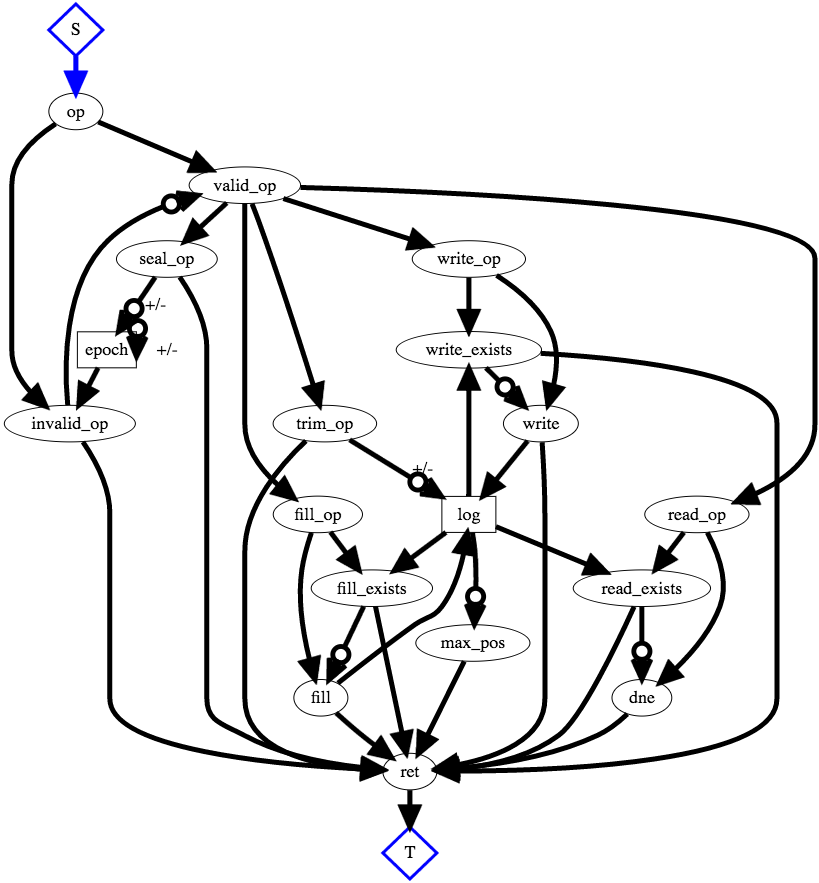
\includegraphics[width=1.0\columnwidth]{Corfu_viz_expanded.png}
%\caption{}
%\label{fig:malacologyx}
%\end{subfigure}
%\end{figure}

%\begin{figure*}[t]
%\begin{subfigure}{.3\columnwidth}
%\centering
%\scalebox{0.45}{
%\begin{tikzpicture}[->,>=stealth',shorten >=1pt,auto,node distance=2.2cm,semithick]
%%\tikzstyle{every state}=[fill=red,draw=none,text=white]
%
%  \node[initial left,state] (A)              {$EG$};
%  \node[state]         (B) [below right of=A] {$CP$};
%  \node[state]         (D) [right of=B]       {$IO$};
%  \node[state]         (C) [above right of=A] {$GC$};
%  \node[state]         (E) [right of=C]       {$US$};
%  \node[state]         (F) [below right of=E] {$Out$};
%
%  \path (A) edge        node [left] {R,W,F} (B)
%            edge        node {T}     (C)
%        (B) edge        node {F}     (C)
%            edge        node {R,W}   (D)
%        (C) edge        node {F,T}   (E)
%        (D) edge        node {W}     (E)
%            edge        node {R}     (F)
%        (E) edge        node {F,T,W} (F);
%\end{tikzpicture}
%}
%\caption{}
%\label{fig:corfu-sm}
%\end{subfigure}\hfill
%\begin{subfigure}{.5\columnwidth}
%\centering
%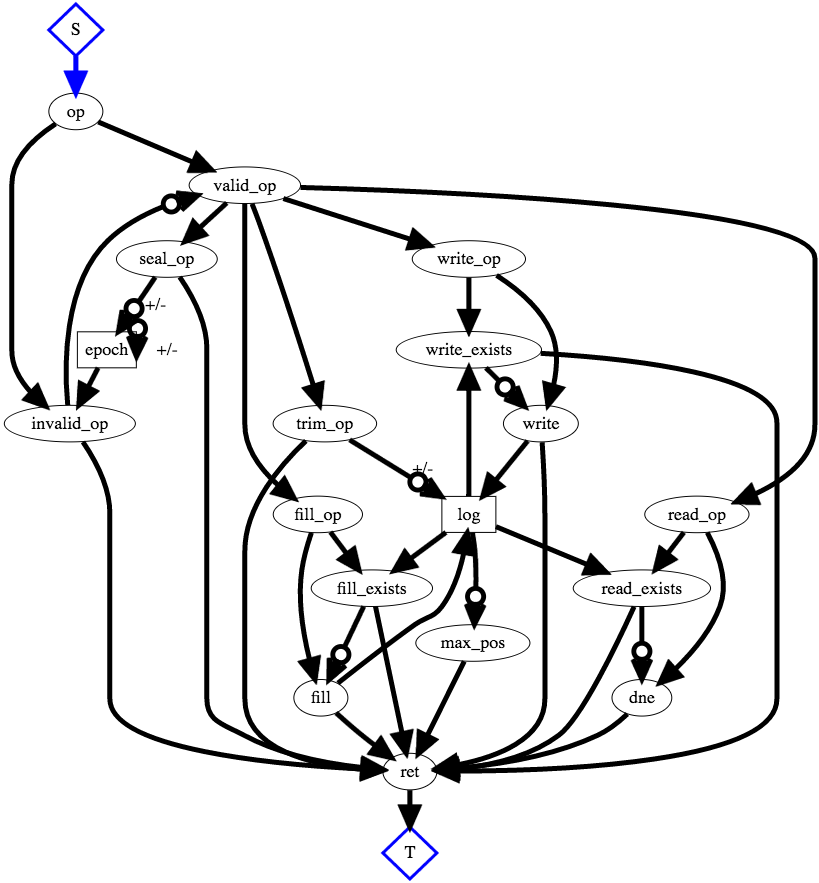
\includegraphics[width=0.95\columnwidth]{Corfu_viz_expanded.png}
%\caption{}
%\label{fig:malacologyx}
%\end{subfigure}\hfill
%\begin{subfigure}{0.9\columnwidth}
%
%\begin{lstlisting}[title={{\bf (c)}}, label=lst:write]
%bloom :write do
%  temp :valid_write <= write_op.notin(found_op)
%  log <+ valid_write{ |o| [o.pos, 'valid', o.data]}
%  ret <= valid_write{ |o|
%    [o.type, o.pos, o.epoch, 'ok'] }
%  ret <= write_op.notin(valid_write) {|o|
%    [o.type, o.pos, o.epoch, 'read-only'] }
%end
%\end{lstlisting}
%\end{subfigure}
%\caption{foo}
%\end{figure*}


\section{Discussion}
\label{sec:opts}

The challenge of navigating the physical design space has served as the
primary source of motivation for selection of a declarative language.  While
our implementation does not yet map a declarative specification on to a
particular physical design, the specification provides a powerful
infrastructure for automating this mapping and achieving other optimizations.
Given the declarative nature of the interfaces we have defined, we can draw
parallels between the physical design challenges described in this paper and
the large body of mature work in query planning and optimization.

Looking beyond standard forms of optimization decisions that seek to select
an appropriate mix of low-level I/O interfaces, data structure selection is an
important point of optimization. For instance in Section~\ref{sec:dspace} we
showed that using the bytestream for metadata management as opposed to the
key-value interface offered superior performance. However the unstructured
nature of the bytestream data model imposes no restrictions on implementation
or storage layout. Integration of common indexing techniques into an optimizer
combined with a performance model will allow our CORFU interface to derive
similar optimizations when appropriate. Similar degrees of freedom can be
imagined when handling other approaches to implementing the CORFU sequencer
service. Given its soft-state nature heavy-weight processes that enforce
durability can be circumvented in favor of shorter code paths that optimize
for throughput and latency.

The Bloom language that we use as a basis for a declarative specificion
language produces a data flow graph that can be used in static analysis. We
envision that this graph will be made available to the OSD and used to reorder
and coalesce requests based on optimization criteria available from a
performance model combined with semantic information from the dataflow. For
example today object classes are represented as black boxes from the point of
view of the OSD execution engine.  Understanding the behavior of an object
class may allow intelligent prefetching. Another type of analysis that may be
useful for optimization is optimistic execution combined with branch
prediction where frequent paths through a dataflow are handled optimistically.

\section{Conclusion}

I can't believe this fits.



{\footnotesize \bibliographystyle{acm}
\bibliography{refs}}



\end{document}
